\preClass{Coordinate Systems}

\videoLink{Section 1.7}{https://www.youtube.com/playlist?list=PLYHZK3b8UFw0MGYUVN9Z4aYof_QgbFw7f}

\begin{enumerate}

\item  Determine whether the function $f$ is even, odd, or neither.
 $$f(x)=4x^3-x$$


\vfill


\item  Evaluate the function for the given values of $x$.
\[
  g(x) =
  \begin{cases}
                                   x+3 & \text{for $x<-1$} \\
                                   x^2 & \text{for $-1 \leq x <2$}   \end{cases}
\]


\begin{enumerate}
\item $g(-2)=$\\
\item $g(-1)=$\\
\item $g(0)=$\\
\item $g(-5)=$\\


\end{enumerate}
\newpage

\item  Graph the piece-wise defined function.
\[
  h(x) =
  \begin{cases}
    2, & \text{for $x \leq -1$}, \\
    2x, & \text{for $x > -1$}.
  \end{cases}
\]
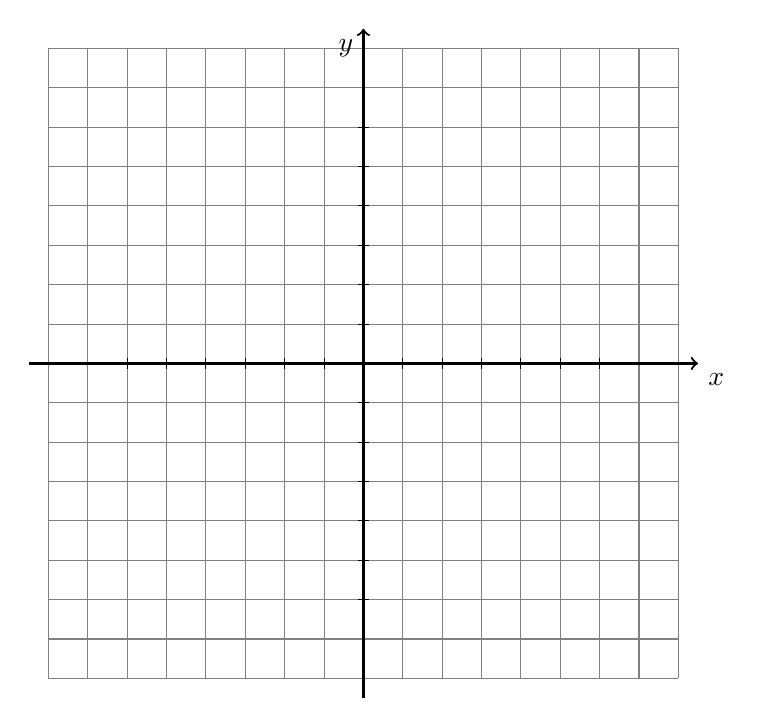
\begin{tikzpicture}[y=.5cm, x=0.5cm,font=\sffamily]
    %% ticks
    \draw[step = 1, gray] (-8,-8) grid (8,8);
    %% axis
    \draw[thick,->] (-8.5,0) -- coordinate (x axis mid) (8.5,0) node[anchor = north west] {$x$};
    \draw[thick,->] (0,-8.5) -- coordinate (y axis mid) (0,8.5) node[anchor = north east] {$y$};
    \foreach \y in {-6,-5,...,-1,1,2,...,6} {
      \draw (2pt, \y) -- (-2pt, \y);
    }
    \foreach \x in {-6,-5,...,-1,1,2,...,6} {
      \draw (\x,2pt) -- (\x,-2pt);
    }
  \end{tikzpicture}



\item  Determine a value of $h$ so that you could sketch the graph of
  the function,
\[
  k(x) =
  \begin{cases}
    h, & \text{for $x \leq -1$}, \\
    2x, & \text{for $x > -1$},
  \end{cases}
\]
without lifting your pencil from the page. Sketch a graph of the
resulting function using the axes below. \\
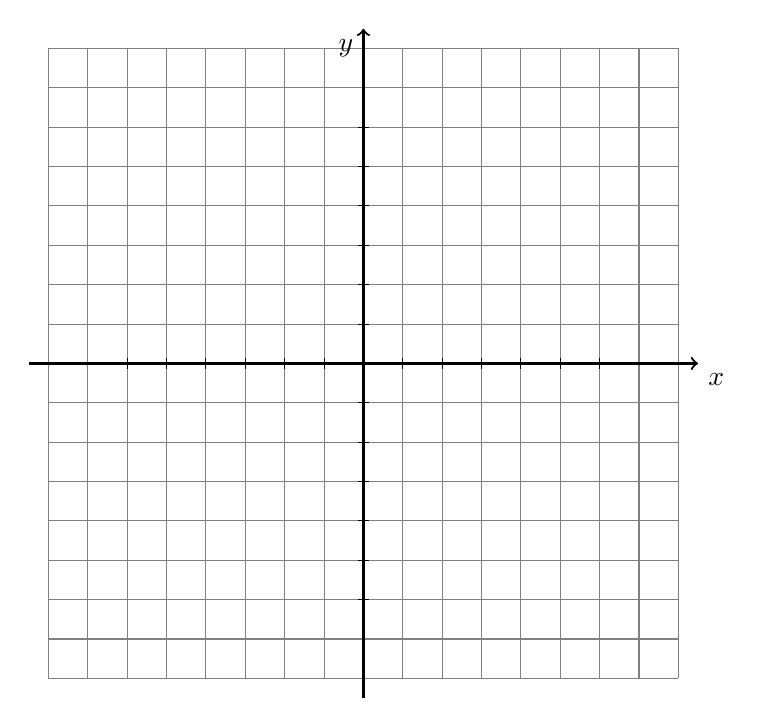
\begin{tikzpicture}[y=.5cm, x=0.5cm,font=\sffamily]
    %% ticks
    \draw[step = 1, gray] (-8,-8) grid (8,8);
    %% axis
    \draw[thick,->] (-8.5,0) -- coordinate (x axis mid) (8.5,0) node[anchor = north west] {$x$};
    \draw[thick,->] (0,-8.5) -- coordinate (y axis mid) (0,8.5) node[anchor = north east] {$y$};
    \foreach \y in {-6,-5,...,-1,1,2,...,6} {
      \draw (2pt, \y) -- (-2pt, \y);
    }
    \foreach \x in {-6,-5,...,-1,1,2,...,6} {
      \draw (\x,2pt) -- (\x,-2pt);
    }

  \end{tikzpicture}







\end{enumerate}


